\newpage
\pagestyle{alternatingstyle}
\chapter{PENDAHULUAN} \label{Bab I}

\section{Latar Belakang} \label{I.Latar Belakang}
Transformasi dunia digital dalam satu dekade terakhir telah membawa dampak besar pada berbagai aspek kehidupan manusia, mulai dari pendidikan, kesehatan, industri kreatif, hingga kesejahteraan sosial. Perubahan ini ditandai oleh munculnya ruang interaksi baru di platform daring, yang memungkinkan masyarakat berbagi informasi, emosi, dan pengalaman hidup dalam berbagai bentuk konten. Perkembangan pesat teknologi informasi dan komunikasi telah mengubah cara manusia berinteraksi, berkomunikasi, dan memproduksi informasi dalam skala global yang menciptakan struktur sosial dan budaya baru serta cara baru dalam berbagi pengetahuan dan pengalaman kolektif. Dalam ranah komunikasi sosial dan interaksi interpersonal, media digital memungkinkan terbentuknya jaringan sosial luas tanpa batas geografis, serta mempercepat penyebaran informasi dan gagasan pada khalayak global \cite{SyakhraniWidijatmoko2024}. 

Seiring dengan perkembangan tersebut, media sosial kini menjadi infrastruktur komunikasi utama dunia. Menurut laporan DataReportal, platform global yang menyajikan analisis digital berbasis data dari mitra riset internasional seperti Kepios, We Are Social, dan Meltwater mencatat bahwa terdapat sekitar 5,04 miliar pengguna media sosial aktif pada awal 2024, atau 62,3\% populasi dunia, dengan pertumbuhan tahunan sebesar +5,6\%, setara dengan 266 juta pengguna baru sepanjang 2023. Rata-rata waktu penggunaan mencapai 2 jam 23 menit per hari , menunjukkan bahwa platform digital kini menjadi ruang publik yang sangat aktif sebagai tempat berbagai bentuk ekspresi diri, termasuk teks, gambar, dan format multimodal seperti meme \cite{datareportal2024_global}\cite {datareportal2024_5billion}. Meme dalam budaya digital adalah unit konten digital yang memiliki karakteristik bersama, dibuat dengan kesadaran terhadap konten lain, serta disebarluaskan, ditiru, dan dimodifikasi oleh banyak pengguna melalui internet \cite{shifman2013memes}. 

% Namun, di balik fungsi hiburan tersebut, tidak semua meme bersifat aman. Sebagian meme dapat mengandung konten sensitif, yang tersirat melalui kombinasi teks dan visual. Sebagai pembanding, tidak semua meme mengandung konten berbahaya. Meme non \textit{self-harm} umumnya hanya menyampaikan humor, kritik sosial, atau ekspresi emosional umum tanpa adanya indikasi sinyal menyakiti diri. 
Dalam konteks komunikasi digital, meme telah menjadi salah satu media ekspresi yang sangat populer karena sifatnya yang ringan, mudah dipahami, dan menghibur. Meme biasanya menggabungkan elemen visual dan teks yang disusun secara kreatif untuk menyampaikan pesan tertentu kepada audiens. Gambar \ref{fig:contohmemenonselfharm} di bawah ini menunjukkan contoh meme yang biasa disebarkan melalui internet. Gambar tersebut diambil dari dataset penelitian yang digunakan dalam penelitian ini. Meme ini menyampaikan pesan yang bersifat umum. 

% Meme ini tidak mengandung indikasi \textit{self-harm} baik dari sisi visual maupun tekstual, sehingga dikategorikan sebagai non \textit{self-harm}.

\begin{figure}[H] % Kalau menggunakan H, posisi gambar akan tepat dibawah teks
    \centering
    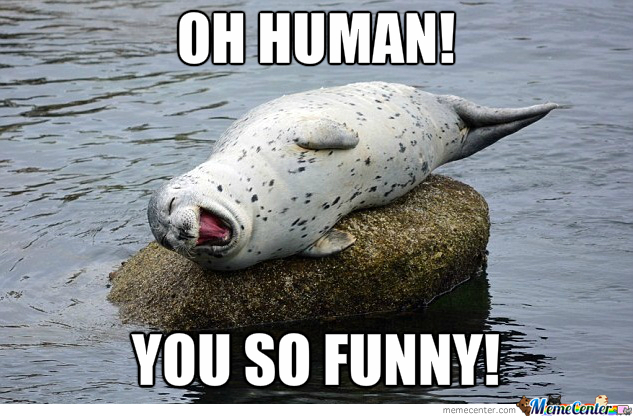
\includegraphics[width=0.6\textwidth]{figure/2088.jpg}
    \caption{Contoh Meme \textit{Non-Self-Harm}}
    \label{fig:contohmemenonselfharm}
\end{figure}


Berbeda dengan meme yang bersifat umum, terdapat juga meme yang mengandung indikasi \textit{self-harm} yang perlu mendapatkan perhatian khusus sebagaimana yang dijelaskan oleh Sharma \textit{et al.} dalam penelitiannya \cite{Sharma2022HarmfulMemes}. \textit{Self-harm} atau perilaku menyakiti diri sendiri secara klinis didefinisikan sebagai tindakan yang dilakukan secara sengaja untuk melukai tubuh sendiri, baik dengan maupun tanpa niat bunuh diri, seperti melukai, membakar, atau bentuk cedera diri lainnya. Perilaku ini umumnya berkaitan dengan kesulitan dalam mengelola emosi, tekanan psikologis, atau pengalaman traumatis, dan menjadi salah satu indikator penting dalam kajian kesehatan mental \cite{NICE_NG225_2022}\cite{who_iris_82c0b4812026}. Dalam digital, \textit{self-harm}  mencakup pada representasi, ekspresi, atau penyebaran konten yang berkaitan dengan perilaku menyakiti diri, baik secara eksplisit maupun implisit \cite{Marchant2017}. Konten ini dapat berfungsi sebagai sarana ekspresi emosional, namun juga berpotensi memperkuat normalisasi atau bahkan mendorong perilaku serupa pada individu lain yang terpapar \cite{seko2015creative}. Hal ini menunjukkan bahwa konten \textit{self-harm} di media sosial bukan hanya fenomena individu, tetapi juga menjadi permasalahan yang memiliki dampak luas secara sosial. 

Dalam penelitian ini, \textit{self-harm} tidak diartikan sebagai diagnosis klinis individu, melainkan sebagai indikasi atau representasi \textit{self-harm} dalam konten meme berdasarkan sinyal multimodal (teks dan visual). Gambar \ref{fig:contohmemeselfharm} di bawah ini menunjukkan contoh meme \textit{self-harm} yang diambil dari dataset penelitian ini dan telah melalui proses anotasi berdasarkan pedoman yang digunakan. Meme ini mengandung indikasi \textit{self-harm} yang diperkuat oleh kombinasi antara elemen visual dan tekstual, sehingga maknanya tidak dapat dipahami hanya dari salah satu modalitas saja.

\begin{figure}[H] % Kalau menggunakan H, posisi gambar akan tepat dibawah teks
    \centering
    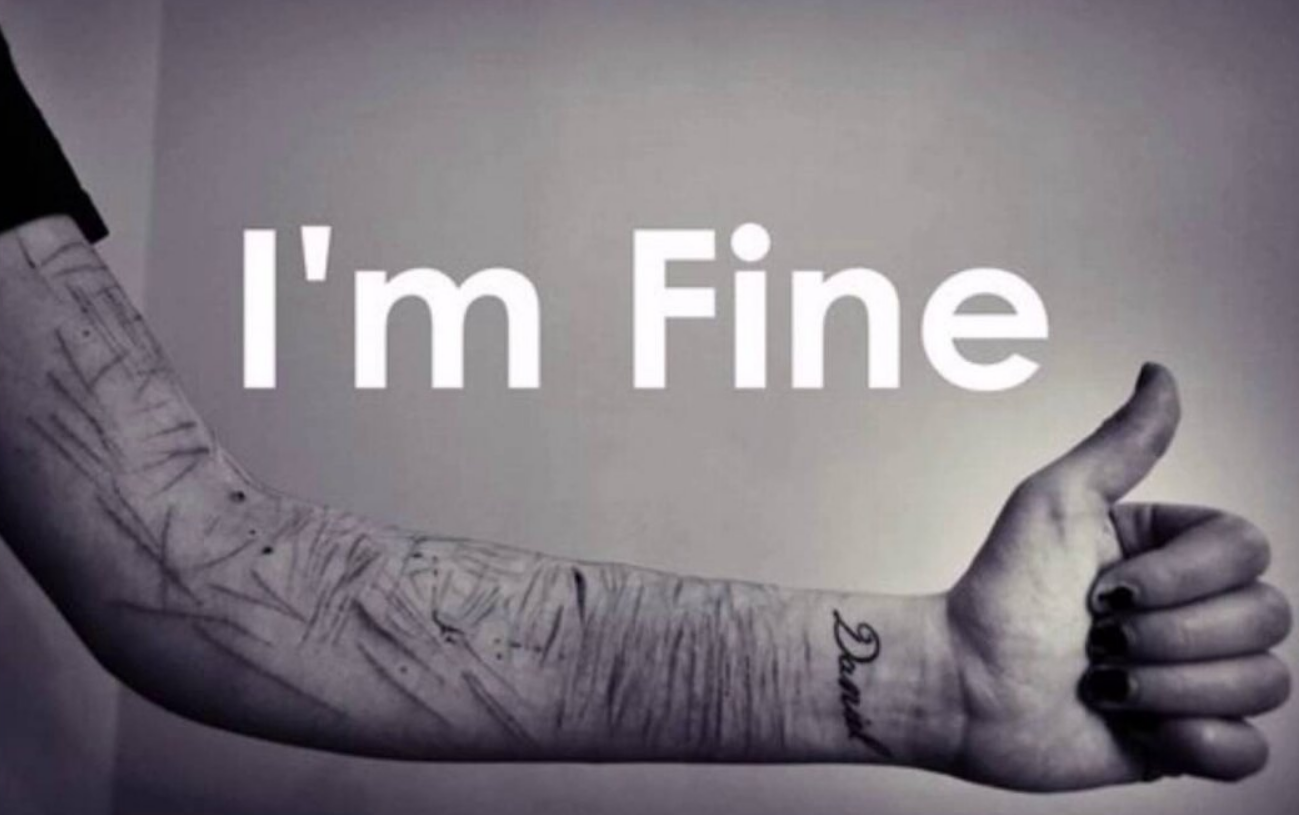
\includegraphics[width=0.5\textwidth]{figure/0492.png}
    \caption{Contoh Meme \textit{Self-Harm}}
    \label{fig:contohmemeselfharm}
\end{figure}


Platform seperti Instagram, Twitter, dan TikTok sering menjadi ruang bagi remaja dan dewasa muda untuk mengekspresikan emosi dan membagikan pengalaman personal, termasuk konten terkait \emph{self-harm}. Studi \textit{intensive monitoring} atau pemantauan harian dan mingguan selama beberapa minggu pada remaja menunjukkan bahwa pada minggu-minggu ketika remaja terpapar konten \textit{self-harm} di media sosial, mereka lebih mungkin mengalami dorongan \textit{non-suicidal self-injury} (NSSI) yaitu tindakan melukai diri sendiri secara sengaja tanpa niat untuk mengakhiri hidup, dan terlibat dalam perilaku tersebut pada periode yang sama, bahkan setelah mengontrol durasi penggunaan media sosial dan gejala depresi \cite{zhang2025social}. Temuan ini menekankan bahwa paparan jenis konten yang muncul di media sosial dapat menjadi faktor risiko langsung yang penting, tidak hanya durasi penggunaan \textit{(screen time)}. Paparan tersebut juga dapat terjadi secara tidak disengaja karena sebagian konten sensitif dapat muncul melalui mekanisme rekomendasi pada \textit{feed} \cite{Sabillillah2024PaparanKonten}. Sebuah survei berskala besar yang dilakukan oleh Samaritans bersama Universitas Swansea menunjukkan bahwa sebanyak 83\% pengguna media sosial pernah direkomendasikan konten bernuansa \emph{self-harm} oleh algoritma \emph{feed}. Rekomendasi tersebut muncul, misalnya, pada halaman \emph{Explore} di Instagram atau \emph{For You} di TikTok, meskipun pengguna tidak secara aktif mencarinya \cite{samaritans2022social}. Temuan ini menunjukkan bahwa isu kesehatan mental pada kelompok usia tersebut merupakan tantangan kesehatan masyarakat yang serius \cite{WHO2025AdolescentMentalHealth}.

% Pada tahun 2024, sebuah meta-analisis terhadap remaja usia 10--19 tahun menemukan bahwa 17,7\% remaja pernah melakukan NSSI, dengan prevalensi sebesar 21,4\% pada remaja perempuan dan 13,7\% pada remaja laki-laki. Data tersebut berasal dari 17 negara yang mencakup wilayah Amerika Utara, Australia, Eropa, dan Asia \cite{denton2024global}. Sementara itu, berdasarkan data \emph{Global Burden of Disease} (GBD) 2021, jumlah kematian akibat \emph{self-harm} secara global mencapai sekitar 746{,}400 kasus pada tahun 2021 \cite{an2025global}. Hal ini menegaskan bahwa \emph{self-harm} masih merupakan isu kesehatan masyarakat yang signifikan di berbagai wilayah dunia. Paparan konten \emph{self-harm} di media sosial bahkan terbukti dapat memprediksi perilaku menyakiti diri dalam satu bulan berikutnya pada populasi muda \cite{arendt2019effects}.


Dalam penelitian ini, meme sebagai bentuk konten digital memiliki karakteristik yang unik. Pesan sering disampaikan secara implisit melalui perpaduan visual dan teks, sehingga pemahamannya bergantung pada hubungan antar-keduanya dan tidak dapat ditafsirkan hanya dari salah satu modalitas saja. Fenomena ini menunjukkan bahwa pemaknaan terhadap meme memerlukan pemrosesan lebih dari satu jenis informasi secara bersamaan. Dalam bidang kecerdasan buatan, pendekatan yang memanfaatkan lebih dari satu jenis sumber data disebut \textit{multimodal learning}, yaitu metode pembelajaran mesin yang memanfaatkan lebih dari satu jenis data seperti teks, gambar, audio, atau video untuk memperoleh pemahaman yang lebih utuh terhadap suatu informasi. Secara konseptual, modalitas merujuk pada cara suatu informasi dialami atau direpresentasikan (misalnya teks dan gambar). Suatu permasalahan disebut multimodal ketika melibatkan lebih dari satu modalitas yang perlu diinterpretasikan dan dihubungkan secara bersama, bukan secara terpisah, agar makna yang muncul dapat dipahami secara utuh \cite{baltrusaitis2018multimodal}. Pendekatan ini menjadi penting dalam analisis konten digital seperti meme, di mana makna sering muncul dari kombinasi antara elemen visual dan teks yang saling melengkapi. 

Penelitian yang dilakukan pada tahun 2021 oleh Kiela \textit{et al.}, meme seringkali menyembunyikan makna yang lebih mendalam yang hanya bisa dipahami dengan menggabungkan konteks visual dan tekstual. Gambar \ref{fig:contohmeme} di bawah ini menggambarkan kalimat \textit{"Look how many people love you"} bisa terlihat tidak berbahaya jika dipisahkan, namun jika dipasangkan dengan gambar padang gurun, maknanya bisa berubah menjadi sesuatu yang lebih negatif. Fenomena ini menggambarkan bagaimana model berbasis unimodal sering kali kesulitan untuk mendeteksi nuansa yang hanya bisa dipahami melalui pemahaman multimodal, yakni gabungan antara teks dan gambar \cite{kiela2020hateful}. Hal ini menunjukkan bahwa pemahaman multimodal menjadi kunci dalam menginterpretasikan makna meme yang bersifat implisit.
\begin{figure}[H] % Kalau menggunakan H, posisi gambar akan tepat dibawah teks
    \centering
    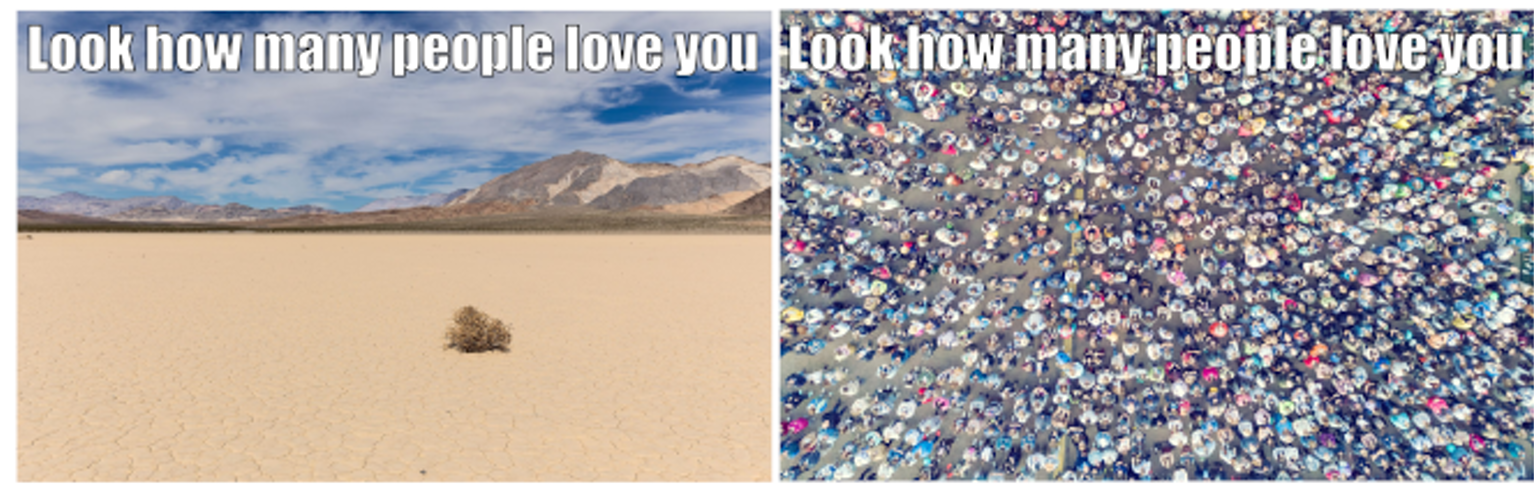
\includegraphics[width=0.9\textwidth]{figure/contohmeme.png}
    \caption{Contoh Meme dengan Makna Tersirat \cite{kiela2020hateful}}
    \label{fig:contohmeme}
\end{figure}

Shah et al. pada tahun 2024  menjelaskan bahwa gambar yang memuat teks membutuhkan pemahaman multimodal mendalam untuk menafsirkan makna tersirat tersebut \cite{shah2024memeclip}. Tantangan ini semakin diperjelas oleh Sharma et al. pada tahun 2022 yang menunjukkan bahwa sebagian besar penelitian masih berfokus pada deteksi \textit{hate speech}, sementara jenis konten berbahaya lainnya seperti \textit{self-harm} dan ekstremisme masih sangat kurang dieksplorasi akibat keterbatasan \textit{dataset} publik \cite{Sharma2022HarmfulMemes}. Untuk mengatasi keterbatasan \textit{dataset} berlabel, pendekatan \textit{pseudo-labeling} digunakan. \textit{Pseudo-labeling} adalah teknik dimana model yang sudah dilatih digunakan untuk memberi label pada data yang tidak berlabel sehingga memperluas \textit{dataset} tanpa memerlukan anotasi manual \cite{lee_pseudo2013}. Teknik ini memungkinkan pelatihan model dengan data tambahan meskipun dengan label yang lemah, yang mengatasi keterbatasan \textit{annotator}. Namun, kondisi ini juga menggarisbawahi adanya kesenjangan riset yang signifikan terkait deteksi meme dengan nuansa \textit{self-harm}. Meskipun berbagai penelitian telah dilakukan dalam bidang deteksi konten berbahaya berbasis multimodal, sebagian besar studi masih berfokus pada kategori seperti \textit{hate speech}, \textit{offensive content}, dan \textit{propaganda}. Sementara itu, konten dengan nuansa \textit{self-harm}, khususnya dalam bentuk meme, masih sangat terbatas untuk diteliti. Selain itu, keterbatasan \textit{dataset} berlabel pada domain ini semakin memperbesar kesenjangan penelitian \cite{zhang2025impact}. Oleh karena itu, diperlukan pendekatan yang mampu memahami hubungan multimodal secara mendalam untuk mendeteksi meme \textit{self-harm} secara lebih akurat.


Seiring dengan perkembangan \textit{multimodal learning}, model pra-latih multimodal seperti \textit{Contrastive Language-Image Pre-training} (CLIP) dirancang untuk mempelajari keterkaitan semantik antara data visual dan tekstual melalui pelatihan pada pasangan gambar dan teks dalam skala besar. Model ini terdiri dari dua \textit{encoder} terpisah, yaitu \textit{image encoder} dan \textit{text encoder}, yang memproyeksikan kedua modalitas ke dalam ruang representasi bersama. CLIP dilatih menggunakan pendekatan \textit{contrastive learning}, yang bertujuan untuk memaksimalkan kesamaan antara pasangan gambar dan teks yang relevan serta meminimalkan kesamaan dengan pasangan yang tidak sesuai. Secara khusus, \textit{image encoder} pada CLIP menunjukkan kemampuan representasi visual yang sangat kuat, karena dilatih menggunakan 400 juta pasangan gambar dan teks dari berbagai domain. Skala data yang besar dan beragam ini memungkinkan model untuk menangkap fitur visual yang kaya dan \textit{generalizable}, sehingga mampu memahami berbagai konteks visual secara lebih akurat \cite{radford2021clip}. Di sisi teks, model \textit{Efficiently Learning an Encoder that Classifies Token Replacements Accurately} (ELECTRA) menawarkan pendekatan yang berbeda dibandingkan metode \textit{Masked Language Modeling} (MLM) yang digunakan dalam \textit{Bidirectional Encoder Representations from Transformers} (BERT). ELECTRA menggunakan skema pelatihan diskriminatif yang dikenal sebagai \textit{replaced token detection}, di mana model dilatih untuk membedakan apakah suatu \textit{token} dalam kalimat merupakan \textit{token} asli atau hasil penggantian oleh \textit{generator}. Pendekatan ini memungkinkan proses pembelajaran terjadi pada seluruh posisi \textit{token} dalam satu waktu, tidak terbatas hanya pada \textit{token} yang di-\textit{masking} seperti pada MLM \cite{clark2020electra}. 

Dalam penelitian ini, pemanfaatan CLIP dan ELECTRA  diintegrasikan melalui skema \textit{intermediate fusion} (\textit{feature-level fusion}), yaitu strategi penggabungan representasi ketika masing-masing modalitas telah dipetakan menjadi fitur tingkat tinggi sebelum dilakukan proses klasifikasi. Pada pendekatan ini, representasi visual yang dihasilkan oleh \textit{image encoder} CLIP dan representasi tekstual dari ELECTRA digabungkan dalam satu ruang fitur, sehingga model dapat mempelajari hubungan semantik lintas modalitas secara lebih mendalam. Pendekatan \textit{intermediate fusion} dipandang relevan untuk analisis meme karena memungkinkan model menangkap interaksi kompleks antara elemen visual dan teks pada level representasi, bukan hanya mengandalkan salah satu modalitas atau menggabungkan hasil keputusan akhir (\textit{late fusion}). Dengan demikian, model diharapkan mampu memahami makna implisit yang sering muncul dalam meme, termasuk konten dengan nuansa sensitif seperti \textit{self-harm} \cite{boulahia2021fusion}. Dengan mempertimbangkan kompleksitas makna pada meme serta potensi dampaknya terhadap kesehatan mental, penelitian ini diharapkan dapat memberikan kontribusi dalam pengembangan sistem deteksi konten \textit{self-harm} berbasis multimodal yang lebih akurat dan kontekstual.

\section{Rumusan Masalah} \label{I.Rumusan Masalah}

Berdasarkan latar belakang yang telah diuraikan di atas, maka permasalahan penelitian dirumuskan sebagai berikut: \par
\begin{enumerate}
    \item Bagaimana membangun model klasifikasi biner dengan menggunakan \textit{Contrastive Language-Image Pre-training} (CLIP) dan \textit{Efficiently Learning an Encoder that Classifies Token Replacements Accurately} (ELECTRA) secara multimodal untuk mengidentifikasi \textit{self-harm} pada meme secara multimodal melalui pendekatan \textit{intermediate fusion}?
    \item Bagaimana pengaruh integrasi representasi visual dari CLIP dan representasi tekstual dari ELECTRA melalui skema \textit{intermediate fusion} untuk meningkatkan pemahaman konteks dalam meme, dibandingkan pendekatan unimodal sebagai \textit{baseline}?
    \item Bagaimana kinerja model multimodal yang diusulkan dalam mendeteksi meme \textit{self-harm} yang dikembangkan dengan menggunakan metrik evaluasi berdasarkan \textit{confusion matrix}?
\end{enumerate}


\section{Tujuan Penelitian} \label{I.Tujuan}
Berdasarkan rumusan masalah yang telah diuraikan di atas, maka tujuan dari penelitian ini adalah: \par

\begin{enumerate}
    \item Mengembangkan model klasifikasi biner berbasis multimodal dengan menggunakan \textit{Contrastive Language-Image Pre-training} (CLIP) dan \textit{Efficiently Learning an Encoder that Classifies Token Replacements Accurately} (ELECTRA) dalam mendeteksi meme yang mengandung indikasi \textit{self-harm} melalui pendekatan \textit{intermediate fusion}.
    \item Menganalisis efektivitas integrasi representasi visual dari CLIP dan representasi tekstual dari ELECTRA melalui skema \textit{intermediate fusion} dalam meningkatkan pemahaman konteks pada meme.
    \item Mengevaluasi kinerja model multimodal yang diusulkan dalam mendeteksi meme \textit{self-harm} dengan menggunakan \textit{accuracy}, \textit{precision}, \textit{recall}, \textit{F1-score}.
\end{enumerate}


\section{Batasan Masalah} \label{I.Batasan}
Batasan masalah dari penelitian adalah sebagai berikut: \par

\begin{enumerate}
    \item Penelitian ini hanya membahas meme sebagai konten digital multimodal yang terdiri dari gambar dan teks. Penelitian tidak mencakup konten berbentuk video, audio, GIF, atau format multimodal lainnya. Pembatasan ini mengikuti karakteristik meme yang membutuhkan pemahaman gabungan antara modalitas visual dan tekstual untuk menangkap makna yang tersirat.

    \item Modalitas teks yang digunakan berfokus pada bahasa Inggris karena model pra-latih yang digunakan dalam penelitian ini dilatih pada domain yang sama dalam bahasa tersebut, sehingga hasilnya lebih konsisten.

    \item Ekstensi gambar yang digunakan dibatasi pada \textit{.jpg/.jpeg}, \textit{.png}, dan \textit{.webp}. Format gambar di luar format tersebut serta konten non-statis (misalnya GIF/video) tidak termasuk dalam ruang lingkup penelitian.

    \item Penelitian ini menerapkan klasifikasi biner, yaitu \textit{self-harm} dan \textit{non-self-harm}. Penelitian tidak mencakup klasifikasi multi-kelas, kategorisasi tingkat keparahan, maupun penilaian risiko klinis/diagnostik.

    \item Definisi operasional kategori ditetapkan sebagai berikut:
    \begin{enumerate}
        \item \textit{Self-harm} dalam penelitian ini merujuk pada representasi \textit{self-harm} dalam konten meme (gambar dan teks), bukan pada diagnosis atau kondisi psikologis individu. 
        \item Dalam penelitian ini, label \textit{self-harm} diberikan hanya pada meme yang sinyal \textit{self-harm}-nya didukung oleh kedua modalitas, yaitu teks dan visual sama-sama merepresentasikan atau menguatkan tema \textit{self-harm}, sehingga konteksnya tidak bergantung pada satu modalitas saja.
        \item \textit{Non-self-harm} adalah meme yang tidak mengandung indikasi \textit{self-harm} pada teks maupun visual. Meme dengan emosi negatif umum tetap termasuk \textit{non-self-harm} selama tidak ada sinyal \textit{self-harm}/keinginan mati.
        \item Penentuan label dilakukan berdasarkan \textit{annotation guideline} berbasis literatur, sehingga hasil klasifikasi merepresentasikan indikasi risiko dalam konten, bukan kebenaran absolut mengenai niat atau kondisi pembuat konten. Oleh karena itu, kemungkinan subjektivitas interpretasi tetap diakui sebagai bagian dari keterbatasan penelitian.
    \end{enumerate}

    \item Penelitian ini menggunakan pendekatan penggabungan fitur tingkat menengah (\textit{intermediate fusion}) untuk mengintegrasikan representasi visual dari CLIP dan representasi tekstual dari ELECTRA. Pendekatan ini dipilih karena memungkinkan model untuk mempelajari hubungan semantik lintas modalitas pada level representasi, yang dianggap lebih relevan untuk analisis meme dibandingkan pendekatan \textit{late fusion} atau \textit{early fusion}.
    
    \item Pedoman anotasi (\textit{annotation guideline}) pada penelitian ini disusun berdasarkan studi literatur terkait definisi \textit{self-harm} dan analisis meme multimodal, tanpa validasi oleh ahli atau klinisi. Oleh karena itu, pedoman ini bersifat operasional dan digunakan khusus dalam penelitian ini, serta menjadi acuan dalam proses pelabelan, termasuk saat pelabelan oleh \textit{Large Language Model} (LLM).
    
    \item Penelitian ini menggunakan pendekatan \textit{weakly supervised learning} dengan pelabelan \textit{ensemble pseudo-labeling} berbasis model/LLM tanpa validasi ahli, sehingga label yang dihasilkan merupakan \textit{weak labels} dan pelatihan model adalah \textit{weakly supervised learning}. \textit{Pseudo-labeling} dipahami sebagai proses pemberian label pada data tak berlabel menggunakan prediksi model, lalu label tersebut digunakan kembali dalam proses pelatihan \cite{lee2013pseudo}. Jika dua model LLM menghasilkan label yang sama, label tersebut digunakan sebagai \textit{pseudo-label}. Jika keduanya berbeda, pelabelan dilakukan secara manual oleh peneliti sehingga tidak semua data bergantung sepenuhnya pada prediksi model LLM yang digunakan. 

    \item \textit{Dataset} penelitian diperoleh dari 
    \begin{enumerate}
        \item Dataset primer yang dikumpulkan secara manual dari sumber konten digital, yaitu platform media sosial yang relevan dengan tema \textit{self-harm}, dan rekayasa dataset meme.
        \item Dataset sekunder yang diperoleh dari sumber terbuka sebagai data tambahan untuk pelatihan model. Sumber terbuka ini dipilih untuk memperluas label \textit{non self-harm} sehingga label \textit{self-harm} tetap menjadi minoritas dalam \textit{dataset}, sesuai dengan karakteristik alami dari fenomena tersebut di ruang digital.
    \end{enumerate}

    \item Penelitian ini dibatasi pada pengembangan dan evaluasi model dalam eksperimen \textit{dataset} penelitian, dan tidak membahas implementasi kebijakan moderasi platform maupun penanganan pengguna secara individual.
    
    \item Evaluasi kinerja model dilakukan menggunakan metrik berbasis \textit{confusion matrix} untuk mengukur kemampuan model dalam mendeteksi meme \textit{self-harm}, tanpa membahas aspek interpretabilitas model atau analisis kesalahan secara mendalam.
\end{enumerate}

\section{Manfaat Penelitian} \label{I.Manfaat}
Berikut adalah manfaat yang diharapkan dari penelitian ini: \par
\begin{enumerate}
    \item Menghasilkan model klasifikasi multimodal berbasis CLIP dan \textit{ELECTRA} dengan pendekatan \textit{intermediate fusion} yang mampu memahami hubungan antara teks dan gambar pada meme, sehingga meningkatkan kemampuan deteksi konten \textit{self-harm} dibandingkan pendekatan unimodal.
    
    \item Menyediakan kerangka metodologi dalam pengembangan model deteksi meme berisiko berbasis multimodal yang dapat dijadikan acuan untuk penelitian lanjutan pada domain serupa, seperti \textit{cyberbullying}, \textit{hate speech}, atau konten berbahaya lainnya.
    
    \item Menghasilkan dataset meme \textit{self-harm} berbasis multimodal (teks dan gambar) melalui pendekatan \textit{pseudo-labeling} untuk mengatasi keterbatasan dataset publik pada domain ini, yang telah diidentifikasi sebagai salah satu tantangan utama dalam penelitian \textit{harmful memes}, serta menyediakan dataset yang dapat menjadi acuan bagi penelitian selanjutnya \cite{Sharma2022HarmfulMemes}.
    
    \item Menyediakan sumber daya penelitian berupa dataset, model, dan \textit{pipeline} eksperimen yang terdokumentasi, sehingga memungkinkan replikasi, evaluasi ulang, dan pengembangan lebih lanjut oleh peneliti lain.
\end{enumerate}


\section{Sistematika Penulisan} \label{I.Sistematika}
Sistematika penulisan berisi pembahasan apa yang akan ditulis disetiap Bab. Sistematika  berupa paragraf yang setiap paragraf mencerminkan bahasan setiap Bab. Dengan demikian, sistematika penulisan ini dirancang untuk memandu pembaca memahami alur logis penelitian dari awal hingga akhir, memastikan setiap bab saling terhubung dan berkontribusi pada pencapaian tujuan penelitian secara keseluruhan. \par
\subsection{Bab I Pendahuluan}
Bab ini memuat penjelasan mengenai latar belakang yang menjadi dasar penelitian ini. Latar belakang tersebut menjelaskan tentang konteks permasalahan yang dihadapi dan urgensi penelitian yang dilakukan. Selanjutnya, disajikan rumusan masalah yang merupakan identifikasi masalah yang ingin diselesaikan melalui penelitian ini. Peneliti juga menguraikan tujuan dari penelitian, batasan ruang lingkup penelitian agar fokus, serta manfaat yang diharapkan dari penelitian ini baik untuk pengembangan ilmu pengetahuan maupun untuk praktik di lapangan. Pada bagian ini juga dijelaskan sistematika penulisan yang memuat susunan dan isi tiap bab yang ada dalam tugas akhir ini.

\subsection{Bab II Tinjauan Pustaka}
Bab ini menyajikan kajian teori yang relevan dengan topik penelitian. Tinjauan pustaka mencakup penelitian terdahulu yang memiliki hubungan dengan penelitian ini, serta teori-teori yang mendasari pokok bahasan penelitian. Dalam bagian ini, peneliti akan mengkaji berbagai literatur yang dapat memberikan pemahaman lebih mendalam terkait topik yang diteliti.

\subsection{Bab III Metodologi Penelitian}
Bab ini berisi penjelasan rinci mengenai metode yang digunakan dalam penelitian ini. Selanjutnya, dijelaskan pula rancangan pengujian yang akan dilakukan untuk mengukur dan menganalisis hasil penelitian. Bagian ini juga mencakup penjelasan tentang  pendekatan yang digunakan, teknik pengumpulan data yang dilakukan, metode analisis data yang digunakan untuk mengolah dan menganalisis data yang telah dikumpulkan.

\subsection{Bab IV Hasil dan Pembahasan}
Bab ini memaparkan hasil pengumpulan data, anotasi data, hasil implementasi dan pengujian yang telah dilakukan dalam penelitian. Peneliti juga menganalisis dan mengevaluasi hasil yang diperoleh untuk memberikan gambaran yang jelas tentang pencapaian tujuan penelitian.

\subsection{Bab V Kesimpulan dan Saran}
Bab ini memaparkan kesimpulan yang diambil berdasarkan hasil analisis dan pembahasan yang telah dilakukan. Peneliti merangkum temuan utama dari penelitian ini dan memberikan saran untuk penelitian lebih lanjut. Saran tersebut bisa mencakup perbaikan atau pengembangan lebih lanjut dari penelitian yang dilakukan, serta rekomendasi yang dapat diambil untuk implementasi di masa depan.
\clearpage
